\documentclass[a4paper, 12pt]{article}
\usepackage[total={17cm,25cm}, top=2.5cm, left=2.5cm, right=2.5cm,  includefoot]{geometry}
\usepackage[utf8]{inputenc}
\usepackage{array}
\usepackage{multirow}
\usepackage{hhline}
\usepackage{gensymb}
\usepackage{graphicx}
\graphicspath{ {} }
\usepackage[czech]{babel}
\usepackage{enumitem}
\usepackage{pdfpages}
\usepackage{amsmath}
\usepackage{verbatim}
\usepackage{listings}
\usepackage{hyperref}
\usepackage{amssymb}


\pagestyle{empty} % vypne číslování stránek




\usepackage[OT2,OT1]{fontenc}
\newcommand\cyr
{
\renewcommand\rmdefault{wncyr}
\renewcommand\sfdefault{wncyss}
\renewcommand\encodingdefault{OT2}
\normalfont
\selectfont
}
\DeclareTextFontCommand{\textcyr}{\cyr}
\def\cprime{\char"7E }
\def\cdprime{\char"7F }
\def\eoborotnoye{\char’013}
\def\Eoborotnoye{\char’003}
\setlength{\parindent}{1em} 
%\setlength{\parskip}{0.5ex}


\begin{document}

\begin{titlepage}
\begin{center}
\Huge
\vspace*{4.5cm}
Algoritmy v digitální kartografii \\
\vspace{0.2cm}

\Large  
Konvexní obálky\\
\vspace{0.2cm}

\normalsize  
Zimní semestr 2018/2019\\
%(oprava: )
\vspace{14cm}
\end{center}

\begin{flushright}
\Large
Tereza Kulovaná \\
Markéta Pecenová \\
\end{flushright}

\end{titlepage}


\pagestyle{plain}     % zapne obyčejné číslování
\setcounter{page}{1}  % nastaví čítač stránek znovu od jedné

\tableofcontents
\newpage

\section{Zadání}
Zadání úlohy bylo staženo ze stránek předmětu \href{https://web.natur.cuni.cz/~bayertom/index.php/teaching/algoritmy-v-digitalni-kartografii}{155ADKG}.

\begin{figure}[h!]
	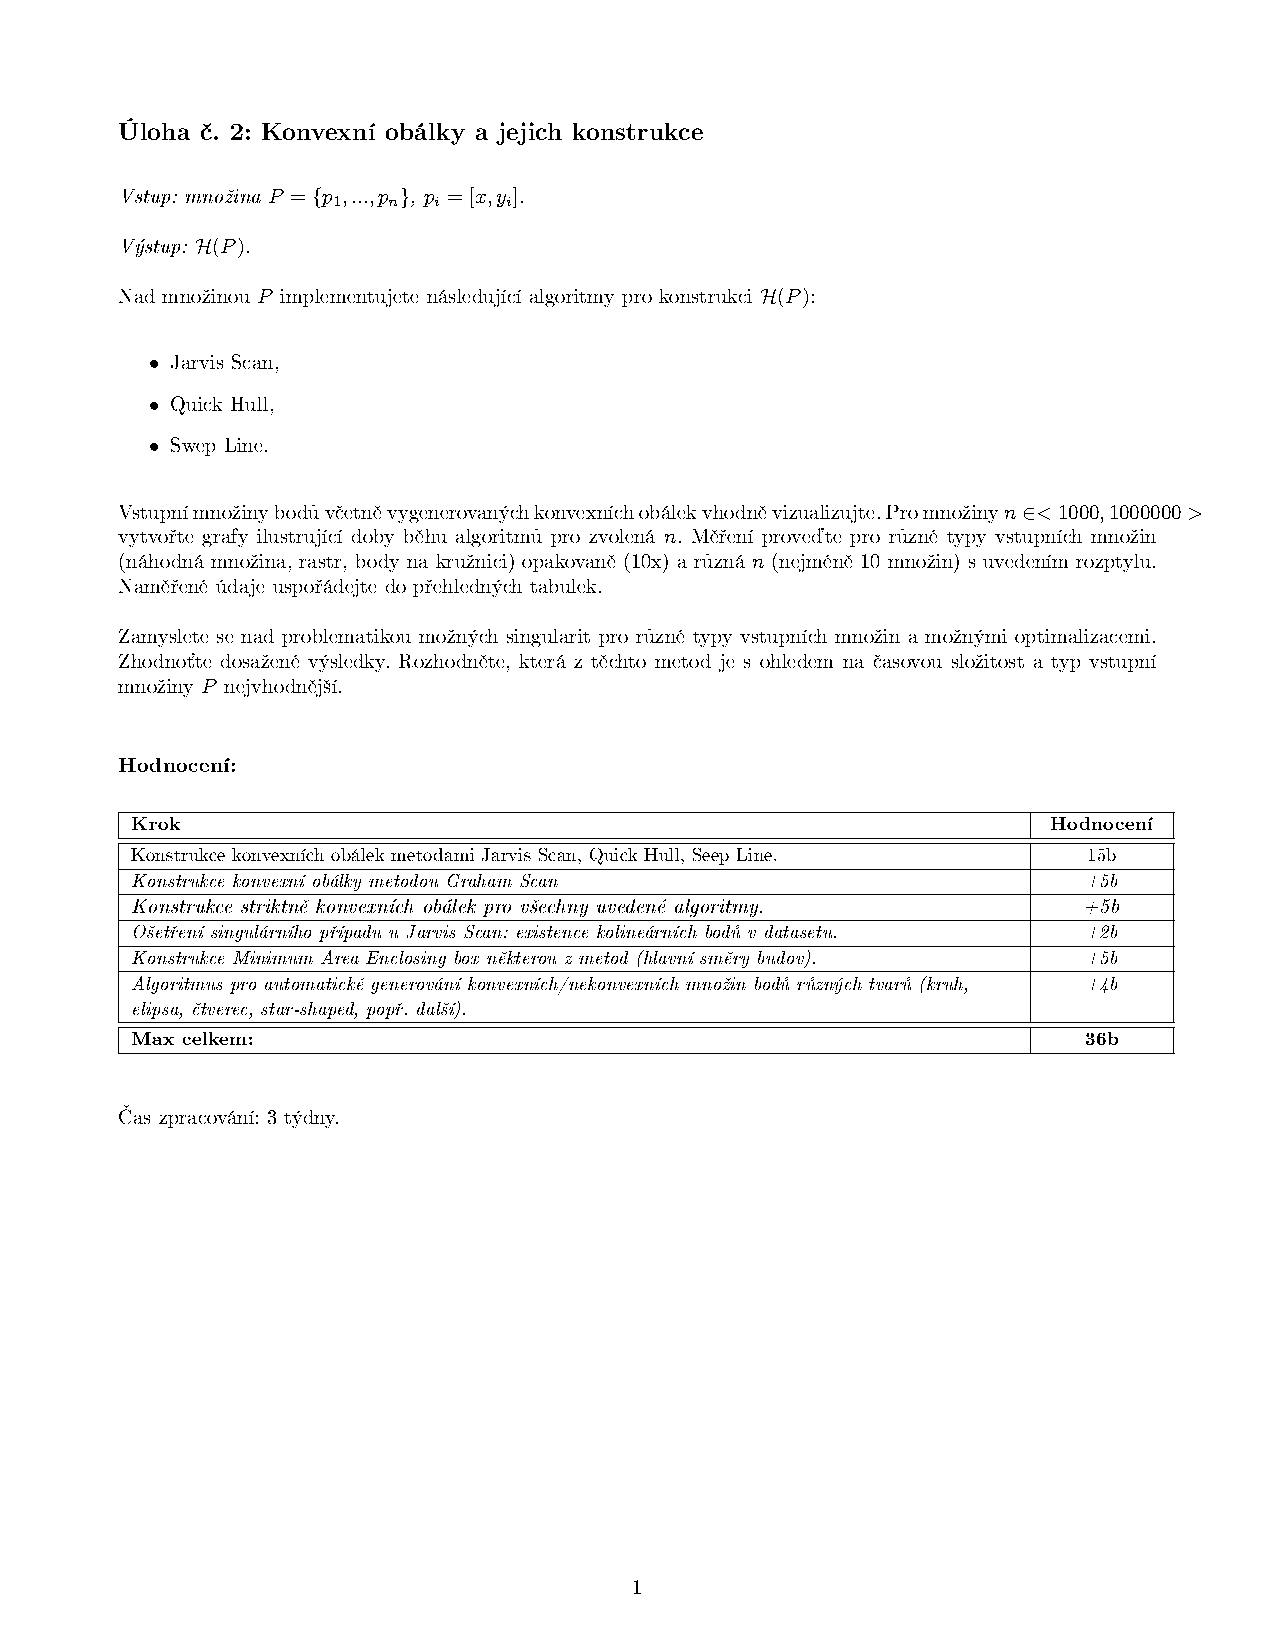
\includegraphics[clip, trim=0cm 10cm 0cm 3cm, width=1.0\textwidth]{./pictures/zadani02.pdf}
\end{figure}

V rámci této úlohy byly implementovány bonusové úlohy č. 2–3. Bonusová úloha č. 5 byla částečně implementována v rámci základního zadání plus navíc bylo přidáno vykreslení elipsy.
\clearpage

\section{Popis a rozbor problému}
Úloha \textbf{Konvexní obálky} se zabývá vytvořením aplikace, která nad vybranou vstupní množinou $S$ vytvoří tzv. konvexní obálku. Konvexní obálka je nejmenší konvexní mnoho\-úhelník $C$ obsahující všechny body z množiny $S$.\\ 

Své využití konvexní obálky nalézají v mnoha oborech. V kartografii se hojně využívají při detekci tvarů a natočení budov pro tvorbu minimálních ohraničujících obdélníků. Dále jsou vhodné pro analýzu tvarů či shluků. Konvexní obálky lze sestrojit v libovolném $\mathbb{R}^n$ prostoru, avšak pro účely této úlohy byl uvažován pouze prostor $\mathbb{R}^2$. V rámci úlohy se testuje výpočetní rychlost použitých algoritmů při konstrukci obálek nad danými vstupními množinami bodů.

\begin{figure}[h!]
	\centering
	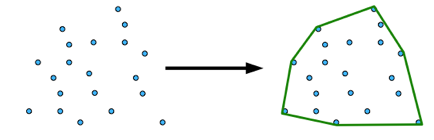
\includegraphics[width=13cm]{./pictures/ch.png}
	\caption{Ukázka konvexní obálky (\href{http://mind.cs.byu.edu/courses/312/projects/project2_files/ConvexHull_python.php}{\textsl{zdroj}})}
\end{figure}

Vzniklá aplikace k tvorbě konvexní obálek využívá tří výpočetních algoritmů: \textit{Jarvis Scan}, \textit{Quick Hull} a \textit{Sweep Line}.

\section{Algoritmy}
Tato kapitola se zabývá popisem algoritmů, které byly v aplikaci implementovány. 

\subsection{Jarvis Scan}
Prvním zvoleným algoritmem je \textit{Jarvis Scan}. Způsob, jakým vytváří konvexní obálku, nápadně připomíná balení dárků (proto je též občas nazýván jako \textit{Gift Wrapping Algorithm}). Mezi nevýhody tohoto algoritmu patří nutnost předzpracování dat a nalezení tzv. pivotu. Algoritmus dále není vhodný pro velké množiny bodů a ve vstupní množině $S$ nesmí být žádné tři body kolineární. Časová náročnost algoritmu je až $O(n^2)$, jeho výhodou však je velmi snadná implementace.\\

Mějme množinu bodů $S$ a pivota $q \in S$, jehož souřadnice Y je minimální ze všech bodů, a přidejme ho do konvexní obálky $H$. Následně do $H$ přidejme takový bod, který s posledními dvěma body přidanými do konvexní obálky svírá maximální úhel. Na začátku výpočtu je nutno inicializovat pomocný bod $s$, jehož souřadnice X je minimální a Y shodná s pivotem $q$, který zajistí dostatečný počet bodů pro výpočet prvního úhlu. Algoritmus končí ve chvíli, kdy nově přidaným bodem do konvexní obálky $H$ je opět pivot $q$. \\

Zjednodušený zápis algoritmu lze zapsat způsobem uvedeným níže:

\begin{enumerate}
\item Nalezení pivota $q$: $q$ = min($y$) 
\item Inicializace pomocného bodu $s$: $s$ = [min($x$), min($y$)]
\item Proveď: $q \in H$
\item Inicializace: $p_{j-1} = s$, $p_j = q$
\item opakuj kroky I–III, dokud $p_{j+1} \neq q$:
\begin{enumerate}[label=\Roman*.]
\item 	Najdi $p_{j+1}$: $\sphericalangle p_{j-1}, p_j, p_{j+1}$ = max
\item 	Proveď: $p_{j+1} \in H$
\item 	Přeindexuj: $p_{j-1} = p_j$, $p_j = p_{j+1}$
\end{enumerate}
\end{enumerate}

\subsection{Quick Hull}
Druhý algoritmus použitý v aplikaci je \textit{Quick Hull}, který k výpočtu konvexní obálky využívá strategii \textit{Divide and Conquer}. Hlavní výhodou algoritmu je jeho rychlost, která není ovlivňována velkým počtem rekurzivních kroků, jak tomu bývá u jiných algoritmů. Časová náročnost výpočtu bývá v nejhorším případě $O(n^2)$ a nastává tehdy, pokud všechny body množiny $S$ náleží konvexní obálce $H$.\\

Mějme body $q_1$, resp. $q_3$, jejichž souřadnice X je minimální, resp. maximální ze všech bodů z množiny $S$. Veďme těmito body pomyslnou přímku, která prostor rozdělí na horní ($S_U$) a dolní ($S_L$) polorovinu. Zbylé body množiny $S$ roztřídíme do daných polorovin podle jejich pozice od přímky. V polorovině následně hledáme bod, který je od dané přímky nejvzdálenější, přidáme ho do konvexní obálky dané poloroviny a přímkami spojíme bod s krajními body přímky předchozí. Proces opakujeme, dokud od nově vzniklých přímek již neexistují vhodné body. Na závěr do konvexní obálky $H$ přidáme bod $q_3$, body konvexní obálky $H_U$ z poloroviny $S_U$, bod $q_1$ a nakonec body konvexní obálky $H_L$ poloroviny $S_L$. Do konvexní obálky $H$ je důležité přidávat body v tomto pořadí, jinak by došlo k nesprávnému vykreslení konvexní obálky $H$. \\

Algoritmus \textit{Quick Hull} se skládá z globální a lokální procedury. Globální část zahrnuje rozdělení množiny na dvě poloroviny a spojení již nalezených bodů konvexních obálek polorovin do jediné $H$. V lokální části se rekurzivně volá metoda, která hledá nejvzdálenější body od přímky v dané polorovině a přidává je do konvexní obálky dané poloroviny $H_i$.\\

\textbf{Globální procedura}:
\begin{enumerate}
\item Inicializace: $H = \emptyset$, $S_U = \emptyset$, $S_L = \emptyset$ 
\item Nalezení $q_1$ = min($x$), $q_3$ = max($x$)
\item Proveď: $q_1 \in S_U$, $q_3 \in S_U$, $q_1 \in S_L$, $q_3 \in S_L$
\item Postupně pro všechna $p_i \in S$:
\subitem Podmínka ($p_i$ je vlevo od $q_1$, $q_3$) $\rightarrow S_U$
\subitem Jinak $ p_i \rightarrow S_L$
\item Proveď: $q_3 \in H$
\item Lokální procedura pro $S_U$
\item Proveď: $q_1 \in H$
\item Lokální procedura pro $S_L$
\end{enumerate}
~\\
\textbf{Lokální procedura nad polorovinou $S_i$}:
\begin{enumerate}[label=\Roman*.]
\item Pro všechny $p_i \in S_i$ kromě bodů přímky:
\subitem Podmínka ($p_i$ vpravo) $\rightarrow$ vzdálenost $d_i$
\subsubitem Podmínka ($d_i > d_{max}$) $\rightarrow d_{max} = d_i$, $p_{max} = p_i$
\item Podmínka (bod $p_{max}$ $\exists$) 
\subitem opakuj krok I. nad první nově vzniklou přímku
\subitem $p_{max} \in H_i$
\subitem opakuj krok I. nad druhou nově vzniklou přímku
\end{enumerate}

\subsection{Sweep Line}
Algoritmus \textit{Sweep Line} neboli \textit{Metoda zametací přímky} je dalším z algoritmů, které byly pro vytváření konvexních obálek implementovány. Jeho princip je založen na imaginární přímce, která se postupně přesouvá zleva doprava nad všemi body množiny $S$. Body, které \uv{přejede}, přidá do dočasné konvexní obálky \={H}, která je následně upravena, aby byla konvexní. Pro tento algoritmus je opět nutné předzpracování vstupních dat (seřadit body $\in S$ podle souřadnice X) s náročností $O(n.$log$(n))$. Další nevýhodou je citlivost algoritmu na singularity, konkrétně na duplicitní body. Ty je vhodné během předzpracování odstranit.\\ 

Algoritmus je postaven na znalosti pozice již vyhodnocených bodů vůči nově přidá\-vanému bodu ukládáním jejich indexů do proměnných $p$ (předchůdce) a $n$ (následník). Zároveň je pro správné fungování algoritmu nutné dodržovat CCW orientaci (proti směru hodinových ručiček). Algoritmus má celkem tři fáze: iniciální a dvě iterativní.\\

V první fázi seřadíme body $p_i$ z množiny $S$ vzestupně podle souřadnice X. Následně z prvních dvou bodů vytvoříme přímku, jejíž koncové body umístíme do konvexní obálky $H$ a indexy bodů umístíme do $n$ a $p$. V první iterativní fázi vyhodnotíme, zda další přidávaný bod leží v horní či dolní polorovině v závislosti na jeho souřadnici Y vzhledem k předchozímu bodu, a opět obousměrně vyhodnotíme indexy $n$ a $p$. Ve druhé iterativní fázi opravujeme dočasnou konvexní obálku \={H} na konvexní $H$ vložením horních a dolních tečen a vynecháním nekonvexních vrcholů.\\

Zjednodušený zápis algoritmu: 
\begin{enumerate}
\item Seřazení $p_i$ podle souřadnice X
\item Pro body $p_0$, $p_1$ proveď:
\subitem $n$[0] = 1, $n$[1] = 0
\subitem $p$[0] = 1, $p$[1] = 0
\item Pro všechna $p_i \in S$, $i > 1$ proveď:
\subitem Podmínka ($y_i > y_{i-1}$) $\rightarrow$ $S_U$: $p$[i] = i-1, $n$[i] = $n$[i-1]
\subitem Jinak $\rightarrow$ $S_L$: $n$[i] = i-1 $p$[i] = $p$[i-1]
\subitem Oprava indexů: $n$[$p$[i]] = i, $p$[$n$[i]] = i
\subitem Dokud $n$[$n$[i]] je vpravo od přímky (i, $n$[i]):
\subsubitem $p$[$n$[$n$[i]]] = i, $n$[i] = $n$[$n$[i]]
\subitem Dokud $p$[$p$[i]] je vlevo od přímky (i, $p$[i]):
\subsubitem $n$[$p$[$p$[i]]] = i, $p$[i] = $p$[$p$[i]]
\end{enumerate}

\section{Problematické situace}
V algoritmu \textit{Sweep Line} bylo nutné ošetřit singularitu, která způsobovala generování nekonvexní obálky. Konkrétně bylo nutné odstranit duplicitní body. Zároveň však toto opatření rapidně navýšilo výpočetní dobu algoritmu, zejména u množiny s vyšším počtem bodů. \\

Podmínka ($p_i == p_j$) $\rightarrow$ bod $p_j$ odstraněn (viz. Obrázek 2)\\

\begin{figure} [h!]
    \centering
      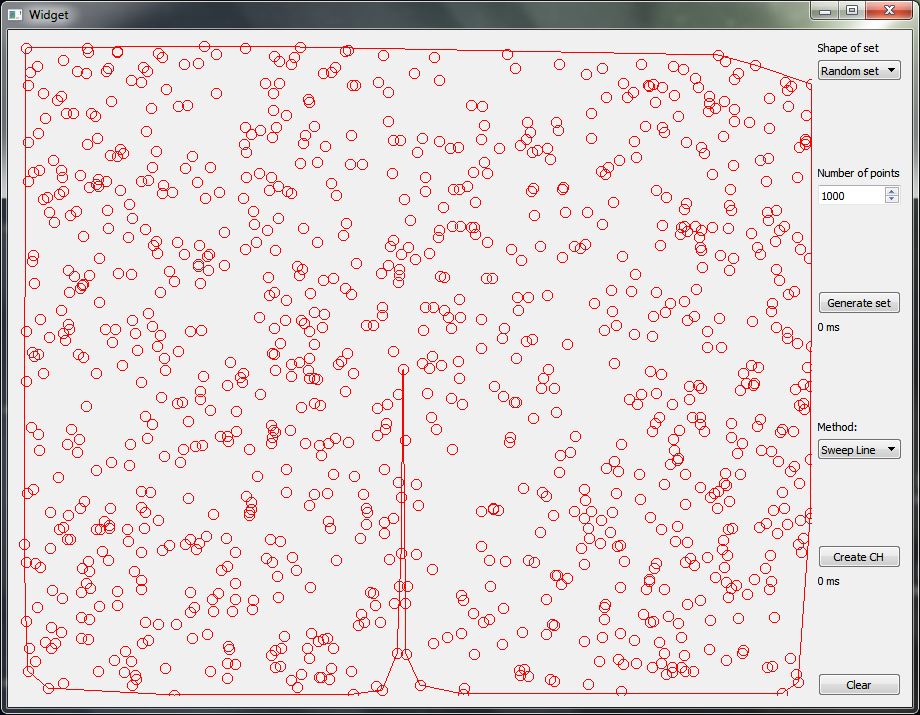
\includegraphics[width=7.5cm]{./pictures/app_sweep_wrong.png}
      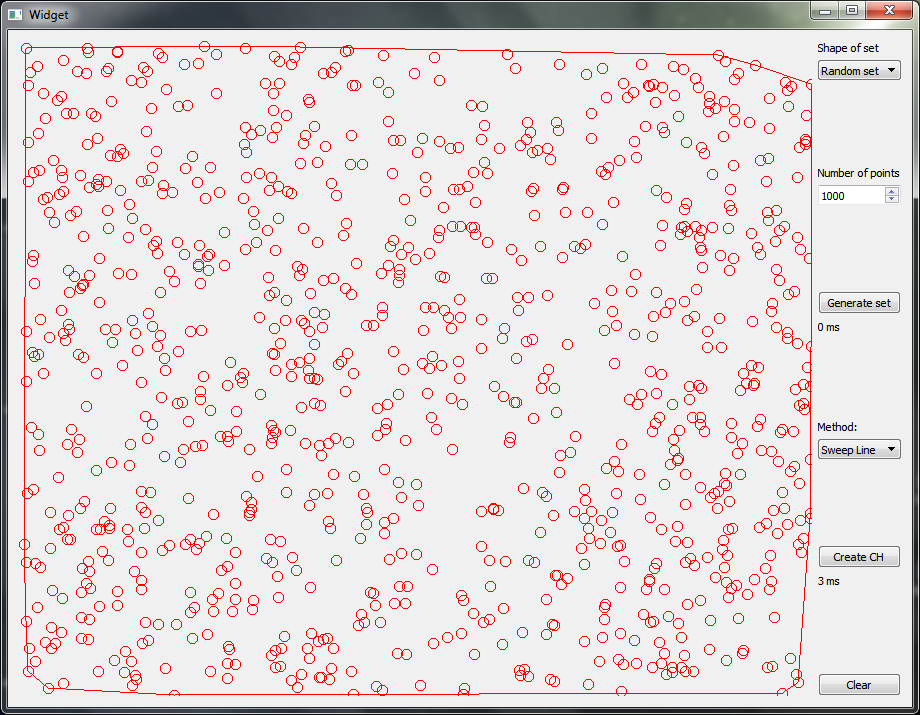
\includegraphics[width=7.5cm]{./pictures/app_sweep_right.png}
      \caption{Neopravený (vlevo) vs. opravený (vpravo) \textit{Sweep Line} algoritmus}
\end{figure}

Algoritmus \textit{Jarvis Scan} generuje špatné výsledky, není-li ošetřeno, že žádné tři body nejsou spolu kolineární. Tento problém se zejména projevoval při generaci setu \textit{Grid}, který jich obsahuje spoustu. Singularita byla ošetřena vypočtením úhlu $\sphericalangle p_{jj}, p_j, p_i$, a pokud byl menší, než stanovená mez $\epsilon$, byl pro další výpočty vybrán bližší z kolineárních bodů.

\begin{itemize}
\item Podmínka ($\sphericalangle p_{jj}, p_j, p_i$) $< \epsilon$
\subitem Podmínka ($d_{p_j,p_i} < d_{min}$) $\rightarrow$ vyber bod $p_i$, $d_{min} = d_{p_j,p_i}$
\end{itemize}

Dalším problémem bylo, jak zajistit, aby byl generovaný rastr pravidelný. To bylo ošetřeno zaokrouhlením počtu vstupních bodů směrem nahoru tak, aby po odmocnění vznikl pravidelný rastr.\\

počet bodů v řádce/sloupci = $roundUp(\sqrt{num\_of\_points})$

\section{Vstupní data}
Aplikace si na základě ručního zadání vstupních parametrů uživatelem sama vygeneruje potřebná vstupní data. Z rozbalovací nabídky \textbf{Shape of set} uživatel volí prostorové uspořádání generované množiny bodů. Na výběr jsou možnosti \textit{Random set}, \textit{Grid} a \textit{Circle}. V kolonce \textbf{Number of points} uživatel volí, kolik bodů bude generováno. Lze tak učinit buď přímým zadáním počtu bodů, nebo zvýšením/snížením počtu bodů o 1000 šipkami na boku. Aplikace omezuje minimální a maximální počet generovaných bodů na interval $\textless$1, 1000000$\textgreater$. Množina bodů se vygeneruje stisknutím tlačítka \textsl{Generate set}.\\

Uživatel má dále možnost volit, jaký výpočetní algoritmus bude použit pro tvorbu konvexní obálky. Rozbalovací nabídka \textbf{Method} nabízí celkem tři výpočetní algoritmy: \textit{Jarvis Scan}, \textit{Quick Hull} a \textit{Sweep Line}. Konvexní obálka je generována stisknutím tlačítka \textsl{Create CH}. Pokud před spuštěním procesu nebyla vygenerována žádná vstupní množina bodů, uživatel je upozorněn chybovou hláškou. 

\section{Výstupní data}
Vygenerovaná množina bodů a její konvexní obálka je vykreslena v grafickém okně aplikace. Aplikace dále vypisuje časy [ms], jak dlouho trvalo generování množiny a jak dlouho nad danou množinou běžel výpočetní algoritmus.\\

V rámci testování byly nad množinami bodů \textit{Random set}, \textit{Grid} a \textit{Circle} postupně spuštěny všechny tři algoritmy. Pro každou množinu a algoritmus byla pro daný počet bodů $n = \{1000, 5000, 10000, 25000, 50000, 75000, 100000, 200000, 500000, 1000000\}$ aplikace spuš\-tě\-na 10x, aby bylo získáno dostatečné množství testovacích dat. Z každé testované množiny bylo tedy získáno celkem 300 testovacích dat. Data byla ukládána do textového souboru a následně zpracována v \textit{Excelu}.

\subsection{Tabulky}
Níže jsou uvedeny průměrné časy běhu algoritmů pro daný počet bodů $n$ z 10 měření pro jednotlivé množiny. Tabulky se všemi naměřenými hodnotami a vypočtenými rozptyly jsou uvedeny v souboru \textit{testing.xlsx}. 

\begin{table}[]
\centering
\begin{tabular}{|c|c|c|c|}
\hline
\multicolumn{4}{|c|}{\textbf{Průměrný čas výpočtu – Random set}}                  \\ \hline
n / algoritmus & Jarvis Scan {[}ms{]} & Quick Hull {[}ms{]} & Sweep Line {[}ms{]} \\ \hline
1000           & 4.5                  & 0.2                 & 1.1                 \\ \hline
5000           & 36.3                 & 1.7                 & 22.5                \\ \hline
10000          & 94.8                 & 3.2                 & 92.6                \\ \hline
25000          & 475.9                & 6.3                 & 539.3               \\ \hline
50000          & 2078.2               & 13.1                & 2091.7              \\ \hline
75000          & 4424.1               & 19.0                & 4450.4              \\ \hline
100000         & 8890.2               & 27.9                & 7818.6              \\ \hline
200000         & 32830.6              & 52.0                & 31694.4             \\ \hline
500000         & 126622.3             & 130.8               & 179290.2            \\ \hline
1000000        & 378372.1             & 245.7               & 635048.4            \\ \hline
\end{tabular}
\end{table}

\begin{table}[]
\centering
\begin{tabular}{|c|c|c|c|}
\hline
\multicolumn{4}{|c|}{\textbf{Průměrný čas výpočtu – Grid}}                        \\ \hline
n / algoritmus & Jarvis Scan {[}ms{]} & Quick Hull {[}ms{]} & Sweep Line {[}ms{]} \\ \hline
1000           & 25.7                 & 0.1                 & 1.0                 \\ \hline
5000           & 284.5                & 0.8                 & 22.6                \\ \hline
10000          & 794.2                & 1.6                 & 84.4                \\ \hline
25000          & 3207.6               & 4.1                 & 462.9               \\ \hline
50000          & 9096.5               & 9.1                 & 1719.1              \\ \hline
75000          & 16612.3              & 14.6                & 3723.1              \\ \hline
100000         & 25434.8              & 19.4                & 6763.6              \\ \hline
200000         & 71724.0              & 33.4                & 27294.5             \\ \hline
500000         & 272534.8             & 89.5                & 179383.6            \\ \hline
1000000        & 567696.9             & 187.1               & 745138.1            \\ \hline
\end{tabular}
\end{table}

\begin{table}[]
\centering
\begin{tabular}{|c|c|c|c|}
\hline
\multicolumn{4}{|c|}{\textbf{Průměrný čas výpočtu – Circle}}                	  \\ \hline
n / algoritmus & Jarvis Scan {[}ms{]} & Quick Hull {[}ms{]} & Sweep Line {[}ms{]} \\ \hline
1000           & 44.7                 & 1.5                 & 1.0                 \\ \hline
5000           & 441.5                & 7.2                 & 17.5                \\ \hline
10000          & 875.0                & 14.0                & 71.1                \\ \hline
25000          & 2382.7               & 34.0                & 389.2               \\ \hline
50000          & 4847.1               & 67.3                & 1502.8              \\ \hline
75000          & 7265.5               & 100.7               & 3468.3              \\ \hline
100000         & 9729.6               & 133.4               & 6254.1              \\ \hline
200000         & 19879.8              & 265.2               & 25542.0             \\ \hline
500000         & 48700.1              & 673.7               & 185213.4            \\ \hline
1000000        & 73295.8              & 1373.5              & 799618.4            \\ \hline
\end{tabular}
\end{table}

\clearpage

\subsection{Grafy}
Níže přiložené grafy zobrazují závislost mezi počtem bodů množiny a průměrným časem výpočtu pro jednotlivé algoritmy. 

%\begin{comment}
\subsubsection{Random set}
\begin{figure}[h!]
	\centering
	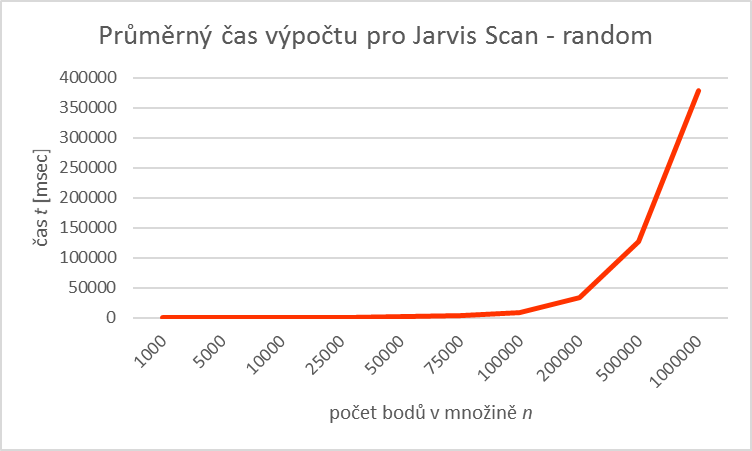
\includegraphics[width=8.5cm]{./pictures/g_rand_js.png}
	\caption{Graf pro Jarvis Scan - random}
\end{figure}

\begin{figure}[h!]
	\centering
	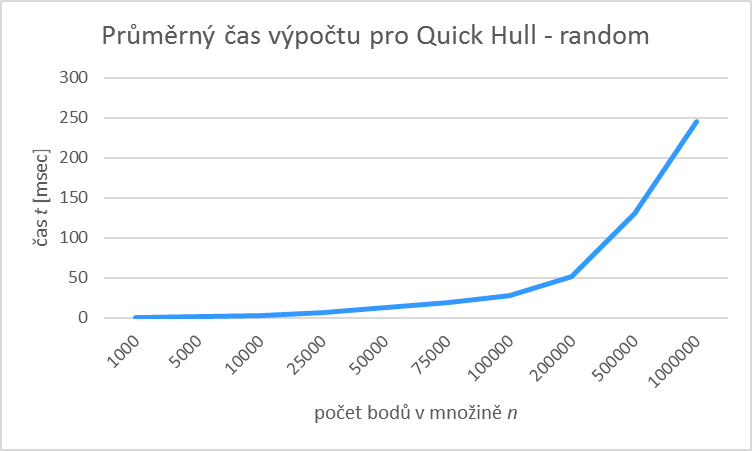
\includegraphics[width=8.5cm]{./pictures/g_rand_qh.png}
	\caption{Graf pro Quick Hull - random}
\end{figure}

\begin{figure}[h!]
	\centering
	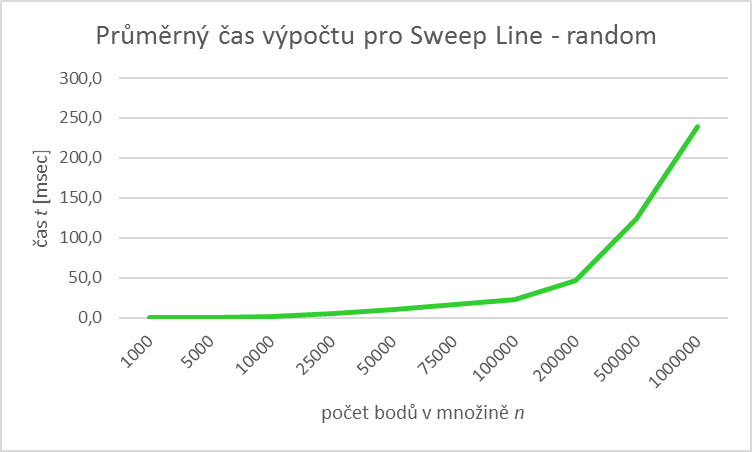
\includegraphics[width=8.5cm]{./pictures/g_rand_sl.png}
	\caption{Graf pro Sweep Line - random}
\end{figure}
\clearpage

\subsubsection{Grid}
\begin{figure}[h!]
	\centering
	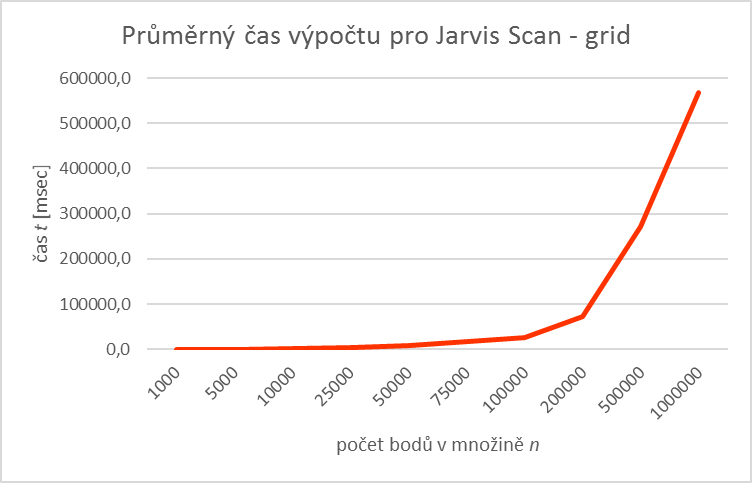
\includegraphics[width=9.5cm]{./pictures/g_grid_js.png}
	\caption{Graf pro Jarvis Scan - grid}
\end{figure}

\begin{figure}[h!]
	\centering
	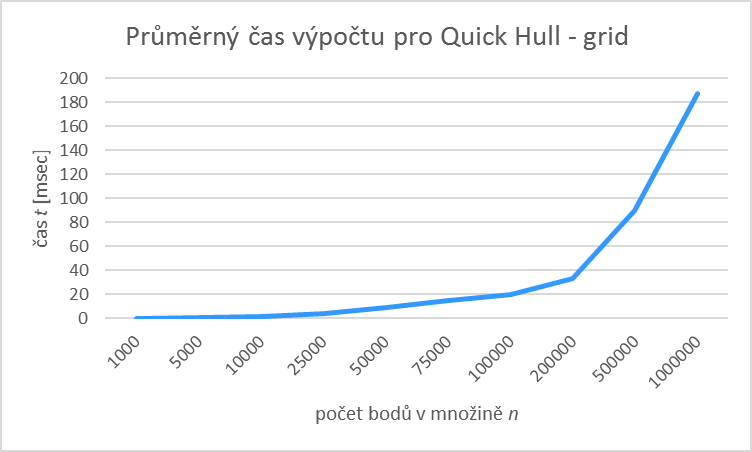
\includegraphics[width=9.5cm]{./pictures/g_grid_qh.png}
	\caption{Graf pro Quick Hull - grid}
\end{figure}

\begin{figure}[h!]
	\centering
	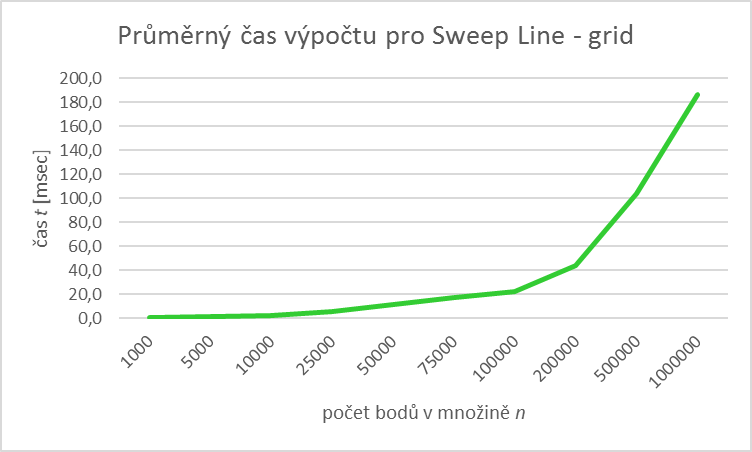
\includegraphics[width=9.5cm]{./pictures/g_grid_sl.png}
	\caption{Graf pro Sweep Line - grid}
\end{figure}
\clearpage

\subsubsection{Circle}
\begin{figure}[h!]
	\centering
	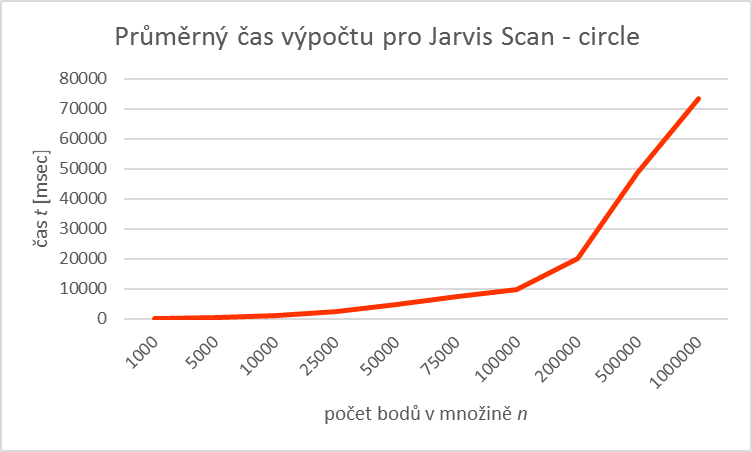
\includegraphics[width=9.5cm]{./pictures/g_circ_js.png}
	\caption{Graf pro Jarvis Scan - circle}
\end{figure}

\begin{figure}[h!]
	\centering
	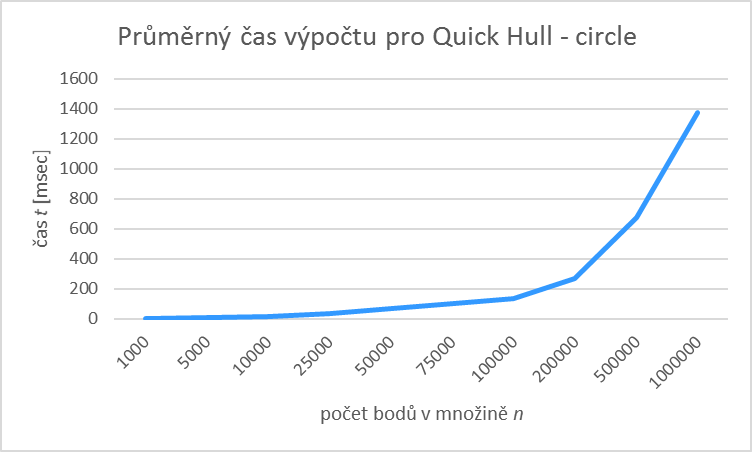
\includegraphics[width=9.5cm]{./pictures/g_circ_qh.png}
	\caption{Graf pro Quick Hull - circle}
\end{figure}

\begin{figure}[h!]
	\centering
	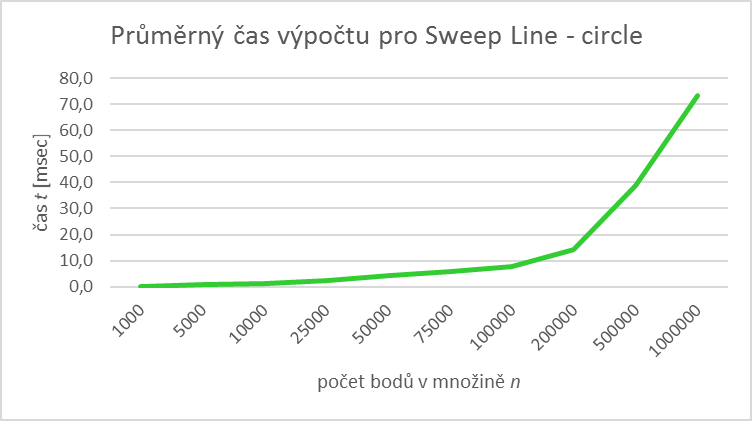
\includegraphics[width=9.5cm]{./pictures/g_circ_sl.png}
	\caption{Graf pro Sweep Line - circle}
\end{figure}
\clearpage

\subsubsection{Porovnání}
\begin{figure}[h!]
	\centering
	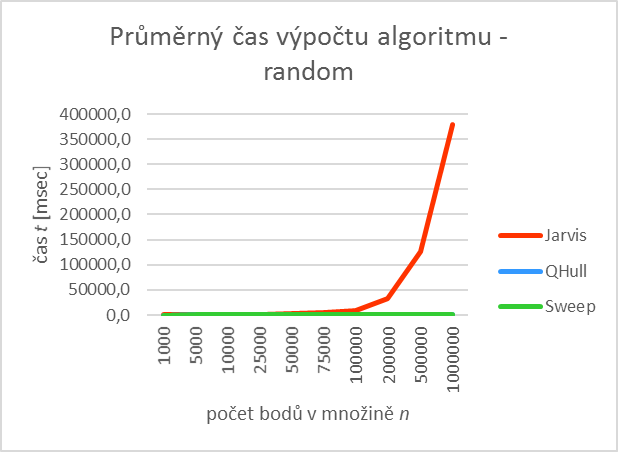
\includegraphics[width=9.3cm]{./pictures/g_rand_all.png}
	\caption{Graf pro množinu \textit{Random}}
\end{figure}

\begin{figure}[h!]
	\centering
	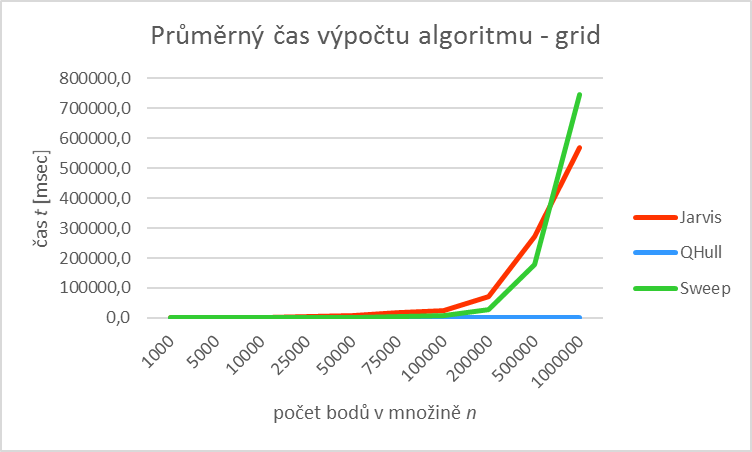
\includegraphics[width=9.3cm]{./pictures/g_grid_all.png}
	\caption{Graf pro množinu \textit{Grid}}
\end{figure}

\begin{figure}[h!]
	\centering
	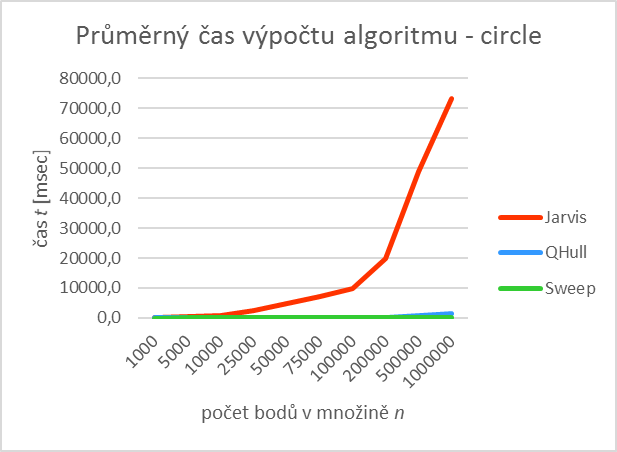
\includegraphics[width=9.3cm]{./pictures/g_circ_all.png}
	\caption{Graf pro množinu \textit{Circle}}
\end{figure}
%\end{comment}

\clearpage
\section{Aplikace}
V následují kapitole je představen vizuální vzhled vytvořené aplikace tak, jak ji vidí prostý uživatel.

\begin{figure}[h!]
	\centering
	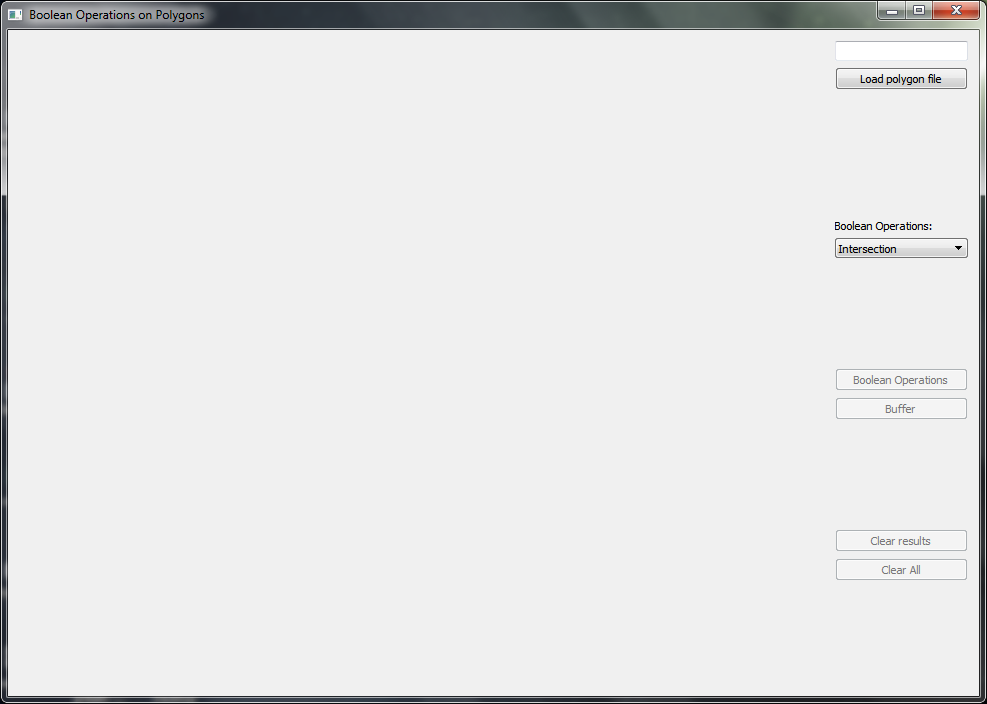
\includegraphics[width=11.5cm]{./pictures/app_default.png}
	\caption{Výchozí vzhled aplikace po spuštění}
\end{figure}

\begin{figure}[h!]
	\centering
	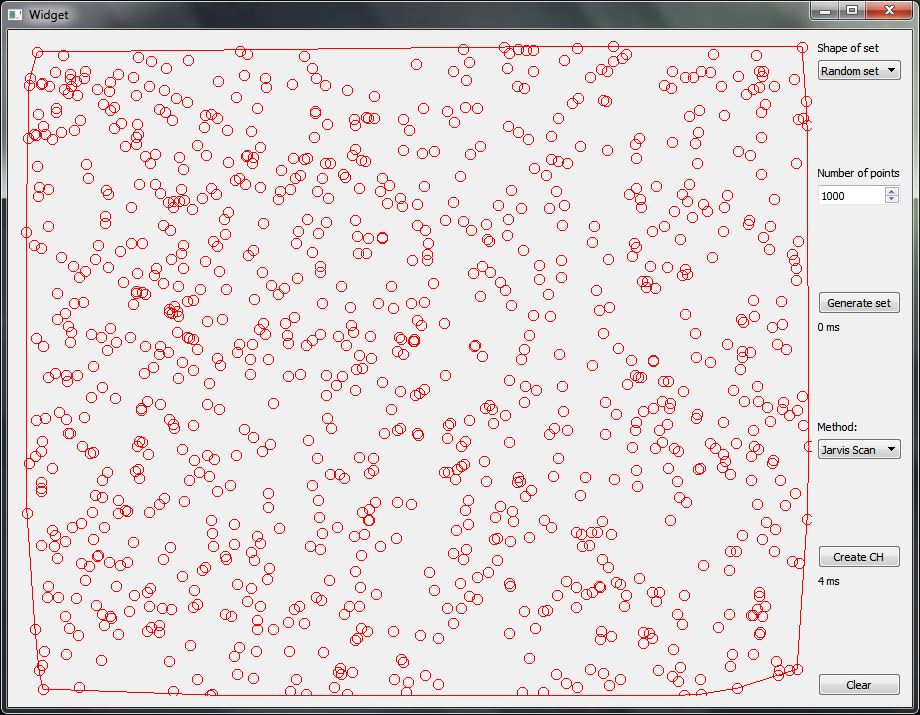
\includegraphics[width=11.5cm]{./pictures/app_random_jarvis.png}
	\caption{Výstup při použití algoritmu \textit{Jarvis Scan} nad množinou \textit{Random} o 1000 bodech}
\end{figure}

\begin{figure}[h!]
	\centering
	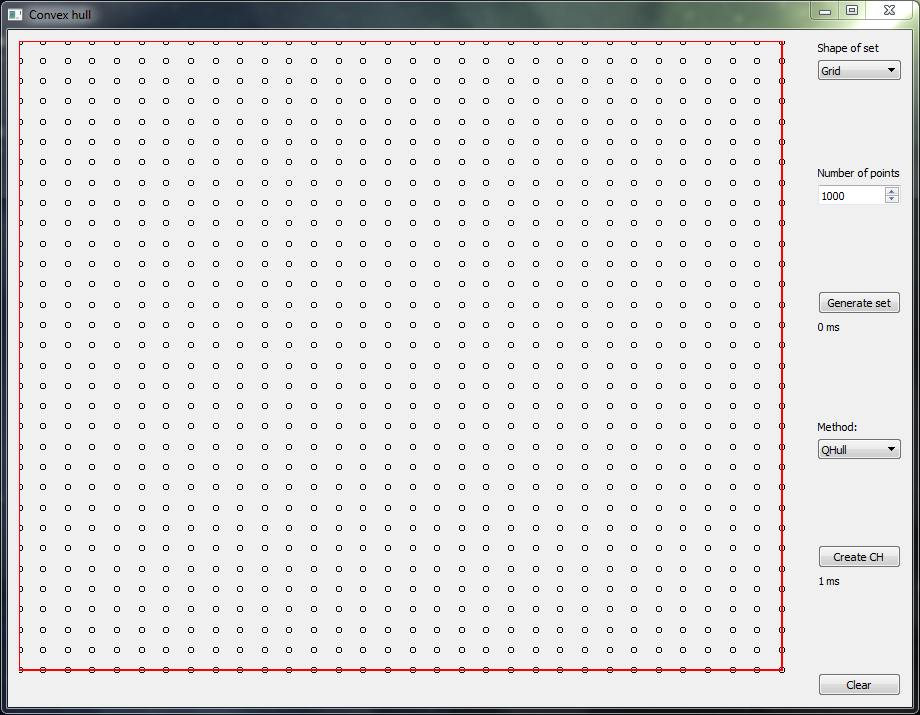
\includegraphics[width=13cm]{./pictures/app_raster_qhull.png}
	\caption{Výstup při použití algoritmu \textit{Quick Hull} nad množinou \textit{Grid} o 1000 bodech}
\end{figure}
~

\begin{figure}[h!]
	\centering
	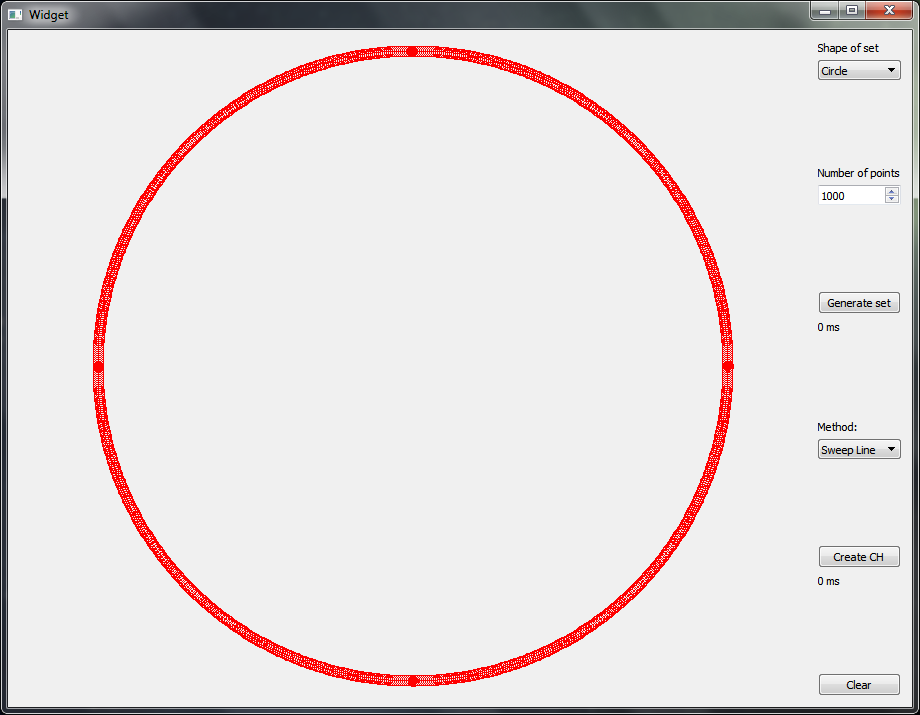
\includegraphics[width=13cm]{./pictures/app_circle_sweep.png}
	\caption{Výstup při použití algoritmu \textit{Sweep Line} nad množinou \textit{Circle} o 1000 bodech}
\end{figure}

\clearpage
 
\section{Dokumentace}
Tato kapitola obsahuje dokumentaci k jednotlivým třídám.

\subsection{Algorithms}
Třída \textit{Algorithms} obsahuje tři základní metody, které nad vstupní množinou bodů vytváří konvexní obálky. Dále obsahuje pomocné metody k výpočtu úhlu mezi dvěma přímkami, metody k určování vztahu bodu a přímky a metodu pro vytvoření striktně konvexní obálky.

\subsubsection*{CHJarvis}
Metoda \textbf{CHJarvis} vytváří konvexní obálku obálku nad vstupní množinou bodů za použití algoritmu \textit{Jarvis Scan}. Na vstupu je vektor bodů třídy \texttt{QPoint}. Návratová hodnota je polygon třídy \texttt{QPolygon}, který obsahuje uspořádané body tvořící konvexní obálku.\\

\textbf{Input}:
\begin{itemize}
\item \textsl{vector} $\textless$\texttt{QPoint}$\textgreater$ $points$
\end{itemize}

\textbf{Output}:
\begin{itemize}
\item \texttt{QPolygon}
\end{itemize}

\subsubsection*{QHull}
Metoda \textbf{QHull} vytváří konvexní obálku obálku nad vstupní množinou bodů za použití algoritmu \textit{Quick Hull}. Na vstupu je vektor bodů třídy \texttt{QPoint}. Návratová hodnota je polygon třídy \texttt{QPolygon}, který obsahuje uspořádané body tvořící konvexní obálku.\\

\textbf{Input}:
\begin{itemize}
\item \textsl{vector} $\textless$\texttt{QPoint}$\textgreater$ $points$
\end{itemize}

\textbf{Output}:
\begin{itemize}
\item \texttt{QPolygon}
\end{itemize}

\subsubsection*{qh\_loc}
Metoda \textbf{qh\_loc} je lokální procedura algoritmu \textit{Quick Hull}, která se volá rekurzivně a hledá nejvzdálenější bod od přímky v dané polorovině a přidává jej do konvexní obálky poloroviny $H_i$. Na vstupu jsou dvě proměnné typu \texttt{int}, které obsahují index počátečního ($s$) a koncového bodu ($e$) dané přímky, vektor bodů vstupní poloroviny třídy \texttt{QPoint} a polygon třídy \texttt{QPolygon}, ve kterém jsou uloženy body konvexní obálky. Návratová hodnota je typu \texttt{void}.\\

\textbf{Input}:
\begin{itemize}
\item \texttt{int} $s$
\item \texttt{int} $e$
\item \textsl{vector} $\textless$\texttt{QPoint}$\textgreater$ $ss$
\item \texttt{QPolygon} $h$
\end{itemize}

\subsubsection*{CHSweepLine}
Metoda \textbf{CHSweepLine} vytváří konvexní obálku obálku nad vstupní množinou bodů za použití algoritmu \textit{Sweep Line}. Na vstupu je vektor bodů třídy \texttt{QPoint}. Návratová hodnota je polygon třídy \texttt{QPolygon}, který obsahuje uspořádané body tvořící konvexní obálku.\\

\textbf{Input}:
\begin{itemize}
\item \textsl{vector} $\textless$\texttt{QPoint}$\textgreater$ $points$
\end{itemize}

\textbf{Output}:
\begin{itemize}
\item \texttt{QPolygon}
\end{itemize}

\subsubsection*{get2LinesAngle}
Metoda \textbf{get2LinesAngle} počítá úhel mezi dvěma přímkami. Na vstupu jsou 4 body typu \texttt{QPoint}, návratová hodnota typu \texttt{double} vrací velikost úhlu v radiánech. Body $p_1$ a $p_2$ definují první přímku, zbylé dva body druhou přímku.\\

\textbf{Input}:
\begin{itemize}
\item \texttt{QPoint} $p_1$ 
\item \texttt{QPoint} $p_2$ 
\item \texttt{QPoint} $p_3$
\item \texttt{QPoint} $p_4$
\end{itemize}

\textbf{Output}:
\begin{itemize}
\item \texttt{double} 
\end{itemize}

\subsubsection*{getPointLineDistance}
Metoda \textbf{getPointLineDistance} počítá nejkratší (kolmou) vzdálenost bodu $q$ od přímky tvořené dvěma body. Na vstupu jsou 3 body typu \texttt{QPoint}, návratová hodnota typu \texttt{double} vrací vzdálenost bodu $q$ od přímky.\\ 

\textbf{Input}:
\begin{itemize}
\item \texttt{QPoint} $q$ 
\item \texttt{QPoint} $a$ 
\item \texttt{QPoint} $b$
\end{itemize}

\textbf{Output}:
\begin{itemize}
\item \texttt{double} 
\end{itemize}

\subsubsection*{getPointLinePosition}
Metoda \textbf{getPointLinePosition} určuje polohu bodu $q$ vzhledem k přímce tvořené dvěma body. Na vstupu jsou 3 body typu \texttt{QPoint}, návratová hodnota je nově definovaný typ \texttt{TPosition}.\\

\textbf{Input}:
\begin{itemize}
\item \texttt{QPoint} $q$
\item \texttt{QPoint} $a$
\item \texttt{QPoint} $b$
\end{itemize}

\textbf{Output}:
\begin{itemize}
\item \texttt{LEFT} $\rightarrow$ bod se nachází vlevo od přímky
\item \texttt{RIGHT} $\rightarrow$ bod se nachází vpravo od přímky
\item \texttt{ON} $\rightarrow$ bod se nachází na přímce
\end{itemize}

\subsubsection*{strictCH}
Metoda \textbf{strictCH} ze vstupního polygonu vytváří striktně konvexní obálku. Přebytečné body konvexní obálky, které leží na přímce, jsou z polygonu odstraněny. Na vstupu má polygon typu \texttt{QPolygon}, návratová hodnota je typu \texttt{void}.\\ 

\textbf{Input}:
\begin{itemize}
\item \texttt{QPolygon} $ch$ 
\end{itemize}

\subsubsection*{getDistance}
Metoda \textbf{getDistance} počítá vzdálenost mezi dvěma body. Metoda byla implementována v rámci ošetření případu kolineárních bodů pro algoritmus \textit{Jarvis Scan}. Na vstupu jsou 2 body typu \texttt{QPoint}, návratová hodnota typu \texttt{double} vrací vzdálenost mezi dvěma body.\\ 

\textbf{Input}:
\begin{itemize}
\item \texttt{QPoint} $a$ 
\item \texttt{QPoint} $b$
\end{itemize}

\textbf{Output}:
\begin{itemize}
\item \texttt{double} 
\end{itemize}

\subsection{Draw}
Třída \textit{Draw} obsahuje metody, které generují a vykreslují vstupní množinu bodů. Dále vykresluje konvexní obálku dané množiny. 

\subsubsection*{paintEvent}
Metoda \textbf{paintEvent} vykresluje vygenerovanou vstupní množinu bodů a její konvexní obálku. Návratová hodnota je typu \textit{void}.

\textbf{Input}:
\begin{itemize}
\item QPaintEvent *e
\end{itemize}

\subsubsection*{setCh}
Metoda \textbf{setCh} slouží k vymazání všech vykreslených dat. Návratová hodnota metody je typu \texttt{void}.

\subsubsection*{generateSet}
Metoda \textbf{generateSet} slouží ke generování vstupní množiny bodů. Na vstupu má čtyři proměnné typu \texttt{int}, které definují prostorové uspořádání generovaných bodů, jejich počet a šířku a výšku kreslící plochy. Metoda defaultně nastavuje počet generovaných bodů na hodnotu 1000 a omezuje maximální možnou hodnotu, kterou lze nastavit, na 1000000 bodů. Rozměr kreslící plochy definuje maximální možné souřadnice, kterých generované body mohou nabývat, a zároveň je z něj odvozován poloměr vykreslované kružnice a elipsy. Návratová hodnota metody je vektor bodů třídy \texttt{QPoint}.\\

\textbf{Input}:
\begin{itemize}
\item \texttt{int} $shape\_index$ (0 $\rightarrow$ random set, 1 $\rightarrow$ grid, 2 $\rightarrow$ circle, 3 $\rightarrow$ ellipse)
\item \texttt{int} $num\_of\_points$ (rozsah: 1000 – 1000000)
\item \texttt{int} $canvas\_width$
\item \texttt{int} $canvas\_height$
\end{itemize}

\textbf{Output}:
\begin{itemize}
\item \textsl{vector} $\textless$\texttt{QPoint}$\textgreater$
\end{itemize}

\subsubsection*{clearAll}
Metoda \textbf{clearCanvas} slouží k vymazání všech vykreslených dat. Metoda neobsahuje žádné proměnné na vstupu a návratová hodnota je typu \texttt{void}.

\subsection{SortByXAsc}
Třída \textbf{SortByXAsc} má na vstupu dva body typu \texttt{QPoint}, návratová hodnota je typu \texttt{bool}. Metoda vrací bod s nižší  souřadnicí X. Mají-li oba body shodnou souřadnici X, vrací bod s nižší souřadnicí Y.\\

\textbf{Input}:
\begin{itemize}
\item \texttt{QPoint} $p_1$
\item \texttt{QPoint} $p_2$
\end{itemize}

\textbf{Output}:
\begin{itemize}
\item 0 $\rightarrow$ bod $p_2$ má nižší $x$ souřadnici
\item 1 $\rightarrow$ bod $p_1$ má nižší $x$ souřadnici
\end{itemize}

\subsection{SortByYAsc}
Třída \textbf{SortByYAsc} má na vstupu dva body typu \texttt{QPoint}, návratová hodnota je typu \texttt{bool}. Metoda vrací bod s nižší  souřadnicí Y. Mají-li oba body shodnou souřadnici Y, vrací bod s nižší souřadnicí X.\\

\textbf{Input}:
\begin{itemize}
\item \texttt{QPoint} $p_1$
\item \texttt{QPoint} $p_2$
\end{itemize}

\textbf{Output}:
\begin{itemize}
\item 0 $\rightarrow$ bod $p_2$ má nižší souřadnici Y
\item 1 $\rightarrow$ bod $p_1$ má nižší souřadnici Y
\end{itemize}

\subsection{Widget}
Metody třídy \textbf{Widget} slouží pro práci uživatele s aplikací. Metody na vstupu nemají žádné parametry a návratové hodnoty jsou typu \texttt{void}.

\subsubsection*{on\_ch\_button\_clicked}
Metoda \textbf{on\_ch\_button\_clicked} na základě uživatelem zvoleného algoritmu generuje konvexní obálku nad vstupní množinou bodů. Metoda zároveň počítá čas [ms], během kterého algoritmus vypočítá konvexní obálku, a vypíše ho do aplikace. Do výpočtu času není zahrnuto vykreslování konvexní obálky.

\subsubsection*{on\_clear\_button\_clicked}
Metoda \textbf{on\_clear\_button\_clicked} vrací aplikaci do výchozí polohy smazáním všeho, co bylo vykresleno. 

\subsubsection*{on\_set\_button\_clicked}
Metoda \textbf{on\_set\_button\_clicked} generuje množinu bodů na základě zadaných vstupních parametrů uživatelem. Metoda zároveň počítá čas [ms], jak dlouho množinu trvalo vygenerovat, a vypíše ho do aplikace.

\clearpage
\section{Závěr}
V rámci úlohy \textit{Konvexní obálky} byla vytvořena aplikace, která nad vstupní množinou bodů vytváří striktně konvexní obálky. V rámci testování, která trvalo dlouho do noci a použitým počítačům dala pořádně zabrat, byla shromážděna data průměrné doby výpočtu striktně konvexní obálky pro jednotlivé algoritmy. Z časových důvodů byly implementovány jen některé bonusové úlohy.\\

Po provedených testech považujeme za nejvhodnější algoritmus pro výpočet konvexní obálky pro všechny typy množin algoritmus \textit{Quick Hull}, a to i přesto, že by měl na kružnici dávat horší výsledky. Ze všech použitých algoritmů je suverénně nejrychlejším, což se výrazně projevilo hlavně na velkých množinách. Výpočet konvexní obálky \textit{Jarvis Scanem} na velkých množinách trval dlouho, avšak překvapila nás rychlost, s jakou se vypořádal s kružnicí. Nicméně výpočet obálky mu i na malých množinách trval o poznání déle než ostatním algoritmům. Jako nevyhovujícím pro všechny typy množin (zejména pokud obsahují velké množství bodů) byl shledán \textit{Sweep Line} algoritmus. Vytvoření konvexní obálky nad množinou o 1 milionu bodů mu trvalo 12-15 minut(pro srovnání, \textit{Quick Hull} to zvládal pod 1.5 s). Vliv na výpočetní dobu jistě má odstranění duplicitních bodů ze vstupní množiny, avšak je to nezbytný krok ke správnému fungování algoritmu.\\

Závěrem by bylo vhodné podotknout, že data z testování nejsou 100\% spolehlivá. Již v průběhu testování bylo zaznamenáno, že doba výpočtu algoritmu velmi závisí na výkonu použitého počítače (rozdíl v rychlostech byl až dvojnásobný) a také na tom, zda jsou v době testování na počítači spuštěny jiné aplikace (např. prohlížeč) nebo se provádí jiné úkony (např. psaní technické zprávy). To může být jednou z příčin vzniku odchylek, které se v datech občas vyskytují. Pro zachování přibližně konzistentních podmínek při testování byly použity dva notebooky s podobným výkonem.\\

Do budoucna by jistě šla rozšířit nabídka generovaných množin bodů a naprogramovat celková automatizace testování. Aktuální verze kódu pro testování obsahovala pouze cyklus na 10 opakování téhož výpočtu. Dále by mohl být naprogramován další výpočetní algoritmus, \textit{Graham Scan}, na který již autorky neměly čas. Mezi pozitivní přínosy úlohy zajisté patří objevení způsobu hromadného exportu grafů z \textit{Excelu} do formátu *.png.

\clearpage

\section{Zdroje}
\begin{enumerate}
\item  \textsl{BAYER, Tomáš. Geometrické vyhledávání bodů} [online][cit. 10. 11. 2018].\\
Dostupné z: \href{https://web.natur.cuni.cz/~bayertom/images/courses/Adk/adk4.pdf}{https://web.natur.cuni.cz}

\item  \textsl{CS 312 - Convex Hull Project} [online][cit. 10. 11. 2018].\\
Dostupné z: \href{http://mind.cs.byu.edu/courses/312/projects/project2_files/ConvexHull_python.php}{http://mind.cs.byu.edu}

\item  \textsl{SOPUCH, Pavel. LaTeX v kostce} [online][cit. 12. 11. 2018].\\
Dostupné z: \href{http://www.it.cas.cz/manual/latex/}{http://www.it.cas.cz}

\item  \textsl{Create LaTeX tables online} [online][cit. 15. 11. 2018].\\
Dostupné z: \href{https://www.tablesgenerator.com/}{https://www.tablesgenerator.com}


\end{enumerate}
\end{document}

%při zmáčknutí create ch se předchozí množina smaže
%popisky u grafů a tabulek
%vyfotit špatny qhull
%dokmentace
%problematické situace: jravis -> jak jsme to vyřešily